\documentclass{article}
\usepackage{amsmath}
\usepackage{amsfonts}
\usepackage{tikz}
\usepackage{qtree}
\usetikzlibrary{automata,arrows}

\begin{document}

\section*{Student Information}
Name: Batuhan Akçan \\
ID: 2580181 \\

\section*{Answer 1}
\subsection*{a)}
$G_1$ represents the language $L = L_1 \cup L_2$ where\\
$L_1 = \{0^n1^n \;|\; n \geq 0\}$ and
$L_2 = \{1^n0^n \;|\; n \geq 0\}$.\\
In other words, $L$ is the language generated by $G_1$.
\subsection*{b)}
Yes, it is ambiguous because the empty string $\epsilon$ has 2 distinct (nonsimilar) derivations:\\
1) $S \rightarrow_{G_1} A \rightarrow_{G_1} \epsilon $\\
2) $S \rightarrow_{G_1} B \rightarrow_{G_1} \epsilon$

\section*{Answer 2}
\subsection*{a)}
The string $a$ has 2 distinct (nonsimilar) derivations:\\
1) $S \rightarrow_{G_2} AB \rightarrow_{G_2} A \rightarrow_{G_2} a$\\
2) $S \rightarrow_{G_2} AB \rightarrow_{G_2} A \rightarrow_{G_2} aA \rightarrow_{G_2} a $.\\
Therefore, the grammar $G_2$ is ambiguous.
\subsection*{b)}
$G_3 = \{V, \Sigma, R', S\}$ where $V = \{a,b,S,A,B\}, \Sigma = \{a,b\}$ and R' is:\\
$S \rightarrow AB$\\
$A \rightarrow aA \;|\; \epsilon$\\
$B \rightarrow bB \;|\; \epsilon$.
\subsection*{c)}
$S \rightarrow_{G_3} AB \rightarrow_{G_3} aAB \rightarrow_{G_3} aB \rightarrow_{G_3} abB \rightarrow_{G_3} abbB \rightarrow_{G_3} abbbB \rightarrow_{G_3} abbb $.\\

\Tree [.S [.A a [.A $\epsilon$ ] ] [.B b [.B b [.B b [.B $\epsilon$ ] ] ] ] ]

\section*{Answer 3}
\subsection*{a)}
\subsubsection*{i)}
Let the grammar that represents $L_1$ be $G_1 = \{V,\Sigma, R, S\}$ where $V = \{S,c,P,d,R,K,L,a,b\},\\ \Sigma = \{a,b,c,d\}$ and R is:\\
$S \rightarrow cP \;|\; dR$\\
$P \rightarrow K \;|\; L$\\
$K \rightarrow aK \;|\; aKb \;|\; a$\\
$L \rightarrow Kb \;|\; aKb \;|\; b$\\
$R \rightarrow aRbb \;|\; e $\\
We can construct a top-down parser $M_1$ where $L(M_1) = L(G_1)$. Since all top-down parsers are deterministic pushdown automata, $M_1$ is also a deterministic pushdown automaton. Since only deterministic context-free languages can be recognized by a deterministic pushdown automata, the language recognized by $M_1$, which is $L_1$, is a deterministic context-free language.
\subsubsection*{ii)}
Let the grammar that represents $L_2$ be $G_2 = \{V,\Sigma, R, S\}$ where $V = \{S,P,R,K,L,a,b,c,d\},\\ \Sigma = \{a,b,c,d\}$ and R is:\\
$S \rightarrow P \;|\; R$\\
$P \rightarrow K \;|\; L$\\
$K \rightarrow aK \;|\; aKb \;|\; ac$\\
$L \rightarrow Kb \;|\; aKb \;|\; cb$\\
$R \rightarrow aRbb \;|\; d $\\
We can construct a top-down parser $M_2$ where $L(M_2) = L(G_2)$. Since all top-down parsers are deterministic pushdown automata, $M_2$ is also a deterministic pushdown automaton. Since only deterministic context-free languages can be recognized by a deterministic pushdown automata, the language recognized by $M_2$, which is $L_2$, is a deterministic context-free language.
\subsection*{b)}
$CF$: context-free,\quad $\overline{CF}$: complement of context-free,\\ $DCF$: deterministic context-free,\quad $R$: regular\\
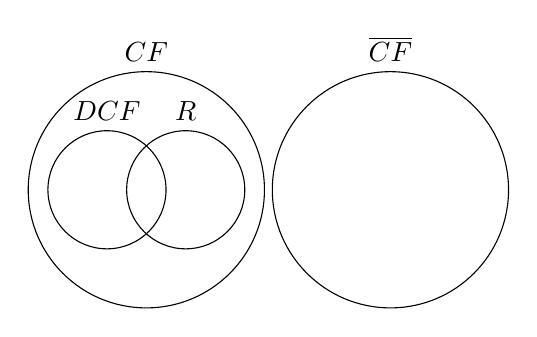
\begin{tikzpicture}

\node [draw,
    circle,
    minimum size =3cm,
    label={90:$CF$}] (A) at (0,0){};
 
\node [draw,
    circle,
    minimum size =3cm,
    label={90:$\overline{CF}$}] (B) at (3.1,0){};
    
\node [draw,
    circle,
    minimum size =1.5cm,
    label={90:$DCF$}] (C) at (-0.5,0){};   
 
\node [draw,
    circle,
    minimum size =1.5cm,
    label={90:$R$}] (D) at (0.5,0){};   
    
\end{tikzpicture}









\end{document}